\chapter{Conclusion}\label{conclusion}


Quantitative genetics and comparative primate functional genomic approaches can be used to disentangle molecular mechanisms regulating gene expression. By identifying genetic variants correlated with a range of molecular functions, quantitative trait loci \emph{(QTL)} mapping studies have contributed to models of how variation percolates through the gene regulatory cascade \citep{degner_dnase_2012, mcvicker_identification_2013, li_rna_2016, pickrell_understanding_2010}. To establish how gene regulatory mechanisms contribute to species divergence, regulatory features are characterized and compared in humans and non-human primates \citep{pai_comparative_2014, romero_widespread_2018, eres_reorganization_2019, blake_comparison_2020, khan_primate_2013, pai_genome-wide_2011, shibata_extensive_2012-1} Both approaches have highlighted the importance of the chromatin accessibility state of cis-regulatory elements, such as promoters and enhancers, in controlling gene expression. However, with the exception of some work on alternative splicing, both lines of research have left co-transcriptional gene regulatory mechanisms that act through variation in mRNA isoforms largely understudied \citep{blekhman_sex-specific_2010, li_rna_2016}. 


Most human genes have the potential to express isoforms terminating at alternative polyadenylation \emph{(APA)} sites with distinct downstream regulatory fates. Usage of an alternative polyadenylation site (PAS) in the 3' UTR can lead to differential inclusion of cis-regulatory elements, such as miRNA binding sites and RNA binding protein motifs. A transcript terminating at an intronic PAS may be subject to decay or be translated into a functional protein. Both 3' UTR and intronic APA can cause isoform specific mRNA stability, mRNA localization, and translation efficiency. (reviewed in Tian, \citep{tian_alternative_2017} Given its downstream consequences, APA likely plays a significant role in gene regulation.

 The complex ways genetic variation can act through APA to shape the transcriptome and proteome have not previously been described. Likewise, how functional divergence in APA between human and chimpanzee genomes contributes to differential expression of genes has not been explored. Thus, to address this gap, I have explored the role of APA in contributing to transcriptome and proteome diversity in a population of human cell lines and in a panel of human and chimpanzee cell lines.
 
 
 
 In Chapter \ref{ch:QTL}, I used a quantitative trait locus \emph{(QTL)} mapping approach to identify genetic variation associated with APA. By measuring QTL sharing between APA and other molecular phenotypes, I determined that genetic variation likely acts through APA to regulate mRNA expression, translation, and protein levels (\ref{fig:abstract}-Top). In Chapter \ref{ch:comp}, I took a comparative primate genomics approach to understand the functional conservation of APA as a regulatory mechanism. Through this analysis, I also gained the power to dissect the details of how APA interacts with other regulatory mechanisms at a finer scale than in Chapter \ref{ch:QTL} (\ref{fig:abstract}-Bottom). While the molecular signals for APA have been characterized, variation in PAS signal sites cannot explain APA variation genome-wide. We hypothesized that co-transcriptional mechanisms, such as RNA polymerase II \emph{(Pol II)} elongation rate, could explain APA variation. In Chapter \ref{ch:netseq}, I tried to formally establish this link in the gene regulatory cascade by identifying genetic variation association with Pol II pausing.  
 
 
 
\begin{figure}
\centering
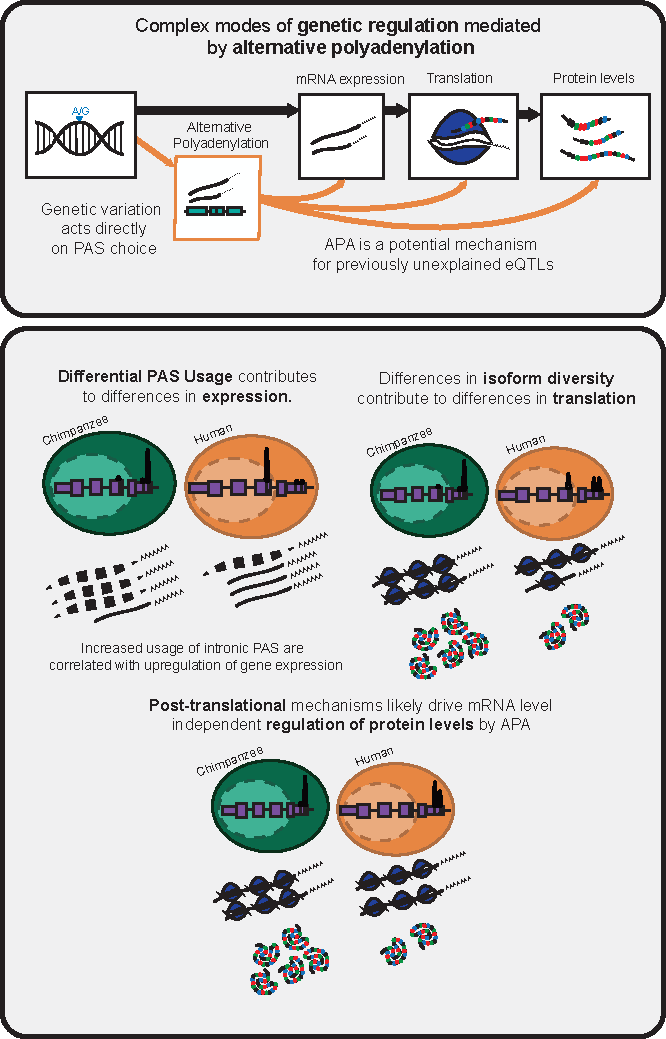
\includegraphics[width=5in]{img/ch05/thesisgraphicalabstract.pdf}
\caption[Graphical Abstract of dissertation]{Graphical abstract to demonstrate major findings in this dissertation. Top: Modes by which genetic variation can influence gene regulation through APA. Bottom: Differences in APA between human and chimpanzee help explain differences in mRNA expression, translation, and protein levels between species. } 
\label{fig:abstract}
\end{figure}

 
 
\section{Genetic underpinning of APA variation}

In Chapter \ref{ch:QTL}, I worked under the supervision of Dr. Yang Li to study the impact of genetic variation on APA. I collected 3' sequencing \emph{(3' Seq)} data on mRNA extracted from whole cells and nuclei of 52 human lymphoblastoid cell lines \emph{(LCLs)}. Using these data, I was able to show that genetic effects on APA largely act on PAS choice. Because we have previously identified genetic variants associated with mRNA expression, translation, and protein levels in the same population, I was able to integrate apaQTLs, eQTLs, riboQTLs, and pQTLs into my analysis. I showed that alleles associated with increased usage of intronic PAS also correlated with decreased mRNA expression. My work suggested that, through usage of intronic PAS and other mechanisms, APA can explain around 20\% of the eQTLs previously unexplained by chromatin variation \citep{li_rna_2016}.  I also identified apaQTLs that were not eQTLs. Some of the apaQTLs that are not significantly associated with expression are correlated with variation in translation, protein levels, or both. Finally, I explored the link between APA and complex traits. I demonstrated that genetic variation surrounding PAS significantly contributes to the heritability of complex immune traits and that 19.3\% of apaQTLs are in high linkage disequilibrium with GWAS loci.  

Throughout my thesis work, a number of groups have recognized the opportunity to study the genetic variation associated with APA  \citep{yang_snp2apa_2019, mariella_length_2019, li_genetic_2019}. My work was novel in that I directly measured PAS usage with 3' Seq rather than estimating usage from traditional RNA sequencing data. While PAS can be inferred from traditional RNA sequencing methods, estimates of usage are imprecise \citep{ha_qapa_2018}.  To our knowledge, we are the only group to measure PAS usage in both nuclear and total mRNA and to conclude that genetic variation largely acts on PAS choice rather than through isoform specific regulation. By detecting apaQTLs in a range of tissues and cancer cell lines, these studies further implicated the role of genetic variation acting through APA to contribute to complex trait variation and disease risk \citep{yang_snp2apa_2019, mariella_length_2019, li_genetic_2019}.

Alternative mRNA splicing and APA are both co-transcriptional gene regulatory mechanisms. Interplay between these two processes contribute to gene regulatory outcomes because splicing and polyadenylation rely on a subset of similar protein complexes competing for space \citep{proudfoot_integrating_2002}. Although I chose not to explore the interplay between mRNA splicing and APA, I used my data to test one interesting hypothesis. Previous studies have implicated the splice factor, U1 snRNP, in protecting introns from premature cleavage and polyadenylation, termed telescripting \citep{kaida_u1_2010, berg_u1_2012, oh_u1_2017}.  Because the U1 snRNP binds to 5' splice sites, I expected some intronic PAS to escape telecripting because they lie in introns with weak 5' splice sites. Supporting this hypothesis, I found an enrichment of intronic PAS in introns with the weakest 5' splice sites. However, the questions of if and how genetic variation can contribute to both alternative splicing and APA remain to be explored.



\section{Functional conservation of APA }

In Chapter \ref{ch:QTL}, I showed that some genetic variation associated with APA is also associated with mRNA expression variation. In Chapter \ref{ch:comp}, I used a comparative genomics approach to further investigate the role of APA in gene regulation.  I concluded that differential expression could be driven specifically by switching between dominant isoforms. However, I did not find evidence that differences isoform diversity contributes to differential expression. I also provided additional evidence that APA contributes to proteomic diversity independent from differences in mRNA levels. 

In Chapter \ref{ch:QTL}, I showed a negative correlation between intronic apaQTL and eQTL effect sizes. Specifically, for several loci, the allele associated with increased intronic PAS usage was also associated with increased mRNA expression. When I examined a similar relationship between human and chimpanzee, I detected a positive correlation between usage of intronic PAS and gene expression. In Chapter \ref{ch:comp}?s discussion, I outlined a set of non-mutually exclusive interpretations for these seemingly inconsistent results. First, increased usage of an intronic PAS could lead to rapid nonstop decay the transcript. Second, usage of an intronic PAS could allow the transcript to evade down regulation through cis-regulatory motifs located in the 3' UTR. While I cannot say for certain which mechanism is more active genome wide, the large effect sizes for 3' UTR differences between species have led me to place more weight on the second interpretation.  


Functional follow of genes with intronic and 3' UTR PAS are necessary to better understand the mechanistic relationship between intronic PAS and mRNA expression. Functional follow up experiments may be complicated because each PAS usage ratio assigned to the same gene is not an independent measurement. Without independent measurements for each site, it is difficult to identify which isoform contributes most to variation in mRNA expression. In other words, it is possible that decreased usage of the 3' UTR sites correlated with decreased mRNA expression, but we detected the intronic relationship as more significant. 


\section{Pol II dynamics to understand co-transcriptional gene regulation}

In Chapter \ref{ch:netseq}, I described a project that we unfortunately could not complete. We optimized native elongation transcript sequencing \emph{(Net-seq)} for human LCLs with the goal of mapping genetic variation to variation in Pol II elongation rate. We concluded that the technology was not advanced enough to answer the questions we intended to address. On a positive note, by optimizing Net-seq, I validated a protocol to extract mRNA from nuclei. In addition, I also demonstrated the usefulness of the wavelet-based Empirical Bayes shrinkage method to de-noise functional genomic data \citep{xing_flexible_2016}. 

Had we been able to quantify Pol II density variation with Net-seq, it would have informed analyses for my other projects. For example, in Chapter \ref{ch:QTL}, I identified genetic variation associated with APA but did not ask more detailed questions about how the variants control APA. Given the evidence that apaQTLs are enriched in regions of elongation and around the PAS that they regulate, I hypothesize that genetic variation associated with Pol II elongation rate are also apaQTLs. If my results had supported this hypothesis, the results would have added to the growing literature about transcription kinetics and APA.

Transcription kinetics have previously been implicated in APA (reviewed in Proudfoot 2016, \citep{proudfoot_transcriptional_2016}). Interestingly, experiments testing for the causal relationship between Pol II elongation rate and PAS usage are inconsistent. On one hand, Pol II mutations leading to a slowdown in elongation resulted in proximal PAS usage, suggesting changes in Pol II elongation speed cause a PAS to be used \citep{pinto_rna_2011, kornblihtt_chromatin_2006, de_la_mata_slow_2003, howe_perturbation_2003}. On the other hand, nascent transcription measurements suggested that cleavage and polyadenylation factors may be responsible for Pol II pausing rather than the other way around. Specifically, Nojima \emph{et al.} measured the density of post-transcriptionally modified Pol lI after the depletion of cleavage and polyadenylation factors, CPSF73 and CstF64. In each knockdown experiment, the authors reported a reduction of Pol II density at transcription end sites. They concluded that Pol II pausing at transcription end sites is dependent on the polyadenylation machinery \citep{nojima_mammalian_2015}. I may have been able to identify the general sharing between genetic effects on Pol II elongation rate and APA; however, additional follow-up would have been necessary to prove causality. 

Recent investigations have implicated DNA methylation in the relationship between Pol II elongation and APA control \citep{nanavaty_dna_2020}. Nanavaty \emph{et al.}, explored the role of DNA methylation and APA by measuring PAS usage in cell lines with normal and heavily depleted methylation profiles. The authors annotated genes whereby methylation of CTCF binding domains directly downstream of proximal PAS prevented usage of proximal PAS in favor of downstream sites. Interestingly, in the demethylated state, the authors reported increased Pol II density at the CTCF region \citep{nanavaty_dna_2020}. The authors concluded that methylation of DNA may contribute to both transcription elongation and APA regulation. Because the authors identified a range of PAS usage changes upon demethylation of PAS regions, their proposed mechanism does not explain APA genome wide. Exploring the relationship between genetic variation associated with DNA methylation levels and apaQTLs may point to additional mechanisms contributing to co-transcriptional transcriptional gene regulation. 

\section{Future directions}

\subsection{Expanding work to new biological processes}

I collected the data presented in Chapters \ref{ch:QTL}- \ref{ch:netseq} from LCLs growing in culture at a steady state. This work represents the first step to understanding the gene regulatory effects of APA, but we need to expand this work further to more cell types and conditions. The methods and analysis pipelines presented here provide a framework for future studies to explore both the genetic underpinnings and evolutionary trajectory of APA. 

A dynamic analysis of how genetic variation impacts APA would add another dimension to our understanding of gene regulatory pathways. As global changes in APA have been characterized for a range of dynamic biological processes, it is possible that genetic effects acting on such processes would be distinct from those identified in steady state. Changes in cellular state correspond with global changes in APA regulation. Ji and Tian detected global 3' UTR shortening upon reprogramming of human and mouse somatic cells to stem cells \citep{ji_progressive_2009}. Consistent with this observation, a number of groups have observed 3? UTR lengthening during development of a range of species \citep{ji_progressive_2009, hilgers_neural-specific_2011, li_dynamic_2012, mueller_alls_2013}. While changes in expression levels of cleavage and polyadenylation factors likely contribute to APA during cellular state changes, the genetic control of these processes is unknown. 

Using the panel of iPSCs established and validated in the Gilad lab, we could identify genetic variation associated with dynamic changes in alternative polyadenylation during cellular differentiation. As a proof of principle, Strober, Elorbany and Rhodes \emph{et al.} detected transient and dynamic eQTLs during differentiation of iPSCs into cardiomyocytes \citep{strober_dynamic_2019}. Their results suggest that transient genetic effects also contribute to complex traits and disease. I expect characterization of APA along a similar time course would contribute to our understanding of the connection between APA, other gene regulatory process, and complex traits.

In Chapter \ref{ch:comp}, I showed that APA is largely conserved between human and chimpanzee. Yet, the small number of divergent PAS that I found helped to inform differences in mRNA expression, translation, and protein levels across species. Given that APA contributes to gene regulatory changes in response to stress, it would be interesting to know if APA is more or less conserved between species in stressful conditions. Also, because humans and chimpanzees have similar heart anatomy but different cardiovascular disease \emph{(CVD)} pathology, it would be interesting to ask if differences in APA upon the stresses associated with CVD contribute to pathological differences \citep{lammey_interstitial_2008, varki_original_2009}. Ward and Gilad subjected human and chimpanzee iPSC derived cardiomyocytes to a hypoxia and re-oxygenation protocol to ask if differences in mRNA expression contribute to CVD phenotypic differences. Of the 32 cleavage and polyadenylation factors, Ward and Gilad measured expression of 20 \citep{sadek_alternative_2019, ward_generally_2019}. Of the 20 genes, 7 showed a conserved response and 1 showed a chimpanzee specific response. If expression of these polyadenylation factors changes in response to hypoxia and reoxygenation, I also expect changes in conserved and species-specific APA. By studying APA conservation or divergence in a similar framework as Ward and Gilad, we may uncover additional gene regulatory mechanisms contributing to differences in CVD pathology. 


3' Seq and apaQTL calling in cancer tissues or cell lines to identify genetic variation associated with intronic PAS usage is an important future direction for my work. In contrast to APA variation associated with 3' UTR length differences, intronic polyadenylation leads to coding changes that may or may not result in functional proteins \citep{tian_alternative_2017, vasudevan_non-stop_2002, yao_coding_2012}. In Chapters \ref{ch:QTL} and \ref{ch:comp}, I described work characterizing the downstream regulatory consequences of intronic polyadenylation. In 2018, Lee \emph{et al.} presented a mechanism for cancer pathogenesis through intronic polyadenylation that leads to partial or full inactivation of tumor suppressor genes \citep{lee_widespread_2018}. In Chapter \ref{ch:QTL}, I identified an apaQTL in the ELL2 gene \emph{(rs56219066)} associated with usage of an intronic PAS that has previously been associated with risk for multiple myeloma \citep{swaminathan_variants_2015}. It is likely that expanding my work to cancer cell lines would lead to additional insight into the ways genetic variation can act through APA to modify cancer risk.

 
Using available RNA sequencing data in cancer cell lines and tissues, apaQTLs associated with 3' UTR length have been identified. Earlier this year, Yang \emph{et al.} released the SNP2APA database with 467,942 cis-apaQTLs and 30,721 trans-apaQTLs identified in 32 cancer types \citep{yang 2020}. Rather than calculating usage of each PAS, the authors tested for genetic variation associated with the percentage of distal polyA site usage index \emph{(PDUI)}. This strategy likely identified apaQTLs associated with 3' UTR length and is a necessary first step toward understanding the role of APA regulation and cancer. 



\subsection{Technical and methodological future directions}

In this dissertation, I relied on correlations and enrichments to draw conclusions of the role of APA in gene regulation. In Chapter \ref{ch:QTL}, I identified genetic variants correlated with variation in APA. I then asked if the same variants are correlated with mRNA expression, translation, and protein variation. Using this strategy, I concluded that genetic variation acts through APA to regulate gene expression. If the work in Chapter \ref{ch:netseq} came to fruition, I would have used a similar approach to relate Pol II elongation rate to differences in APA and splicing. In Chapter \ref{ch:comp}, I suggested APA may be driving differences in gene regulation between species based on enrichments of statistically significant differences between species in each of the tested molecular phenotypes. 

While correlations and enrichments help us gain important insight, I was not able to report causation or the percent of variation explained by APA in other regulatory phenotypes. Mediation analysis tests if an independent variable causes a mediator and if the mediator causes the outcome. For example, regulatory QTL and comparative genomic studies, mediation analyses have been used to test if genetic variation causes changes in a molecular mechanism as a consequence of differences in gene expression \citep{pierce_co-occurring_2018, park_bayesian_2017, blake_comparison_2020, eres_reorganization_2019}. We have methods for mediation analysis when effect sizes for the mediator and outcome are measures on the same scale. For example, DNA methylation and mRNA expression are both measured linearly, as a sum of genomic reads. However, APA is a ratio of reads and is thus on a different scale than gene expression phenotypes, including mRNA and protein expression. New mathematical models are necessary to incorporate effect sizes measured as ratios into traditional mediation frameworks. 


Long read mRNA sequencing with Pacific Biosciences \emph{(PacBio)} SMRT technology or Oxford Nanopores Ion technology presents a great opportunity for studying APA \citep{amarasinghe_opportunities_2020}. By capturing and sequencing full transcripts, we would be able to detect PAS with higher confidence. In addition, by sequencing full transcripts, we would also be able to connect APA to alternative splicing \citep{amarasinghe_opportunities_2020, reimer_rapid_2020}. However, long read sequencing has a higher per-base error rate and may be subject to mapping errors due to template-switching artifacts \citep{balazs_template-switching_2019}. Thus, it is likely that combining long and short read sequencing may provide more confidence for PAS detection and quantification. As a small part of my dissertation work, I submitted a subset of the human LCLs that I used in Chapter \ref{ch:QTL} for PacBio Iso-seq sequencing. While these data have yet to be fully analyzed, I hope that future work will combine the data published with this dissertation with the PacBio dataset to develop best practices for PAS detection and quantification.


\section{Concluding remarks}

Exploration of gene regulation at an isoform level adds an additional layer of complexity to our understanding of gene expression. While many groups have started to study the regulatory causes and effects of alternative splicing, less has been done to understand APA genome wide. This dissertation and the resulting publications are an attempt to begin filling this gap. I identified genetic variation associated with APA in order to test if APA differences contribute to differences in mRNA expression, translation, and protein levels. I then took a comparative genomic approach to further disentangle the relationship between APA and gene regulation. In doing so, I helped to fill in some of the many remaining gaps in our ability to read the gene regulatory code as a way to understand human complex traits and diseases. 

